\begin{figure}[ht]
	\begin{subfigure}[b]{0.32\linewidth}
		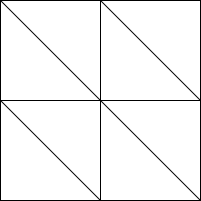
\includegraphics[width=\linewidth]
		{data/synthetic_meshes/square_tesselation_2tri_Dirac_delta_1_v9_f8_wireframe.png}
		\caption{$r=1$, wireframe}\label{fig:sq2.a}
	\end{subfigure}
	\begin{subfigure}[b]{0.32\linewidth}
		\includegraphics[width=\linewidth]
		{data/synthetic_meshes/square_tesselation_2tri_Dirac_delta_1_v9_f8_funcvals_0iter_crop.png}
		\caption{$r=1$, $c=0$}\label{fig:sq2.b}
	\end{subfigure}
	\begin{subfigure}[b]{0.32\linewidth}
		\includegraphics[width=\linewidth]
		{data/synthetic_meshes/square_tesselation_2tri_Dirac_delta_1_v9_f8_funcvals_1iter_crop.png}
		\caption{$r=1$, $c=1$}\label{fig:sq2.c}
	\end{subfigure}

	\bigskip
	\begin{subfigure}[b]{0.32\linewidth}
		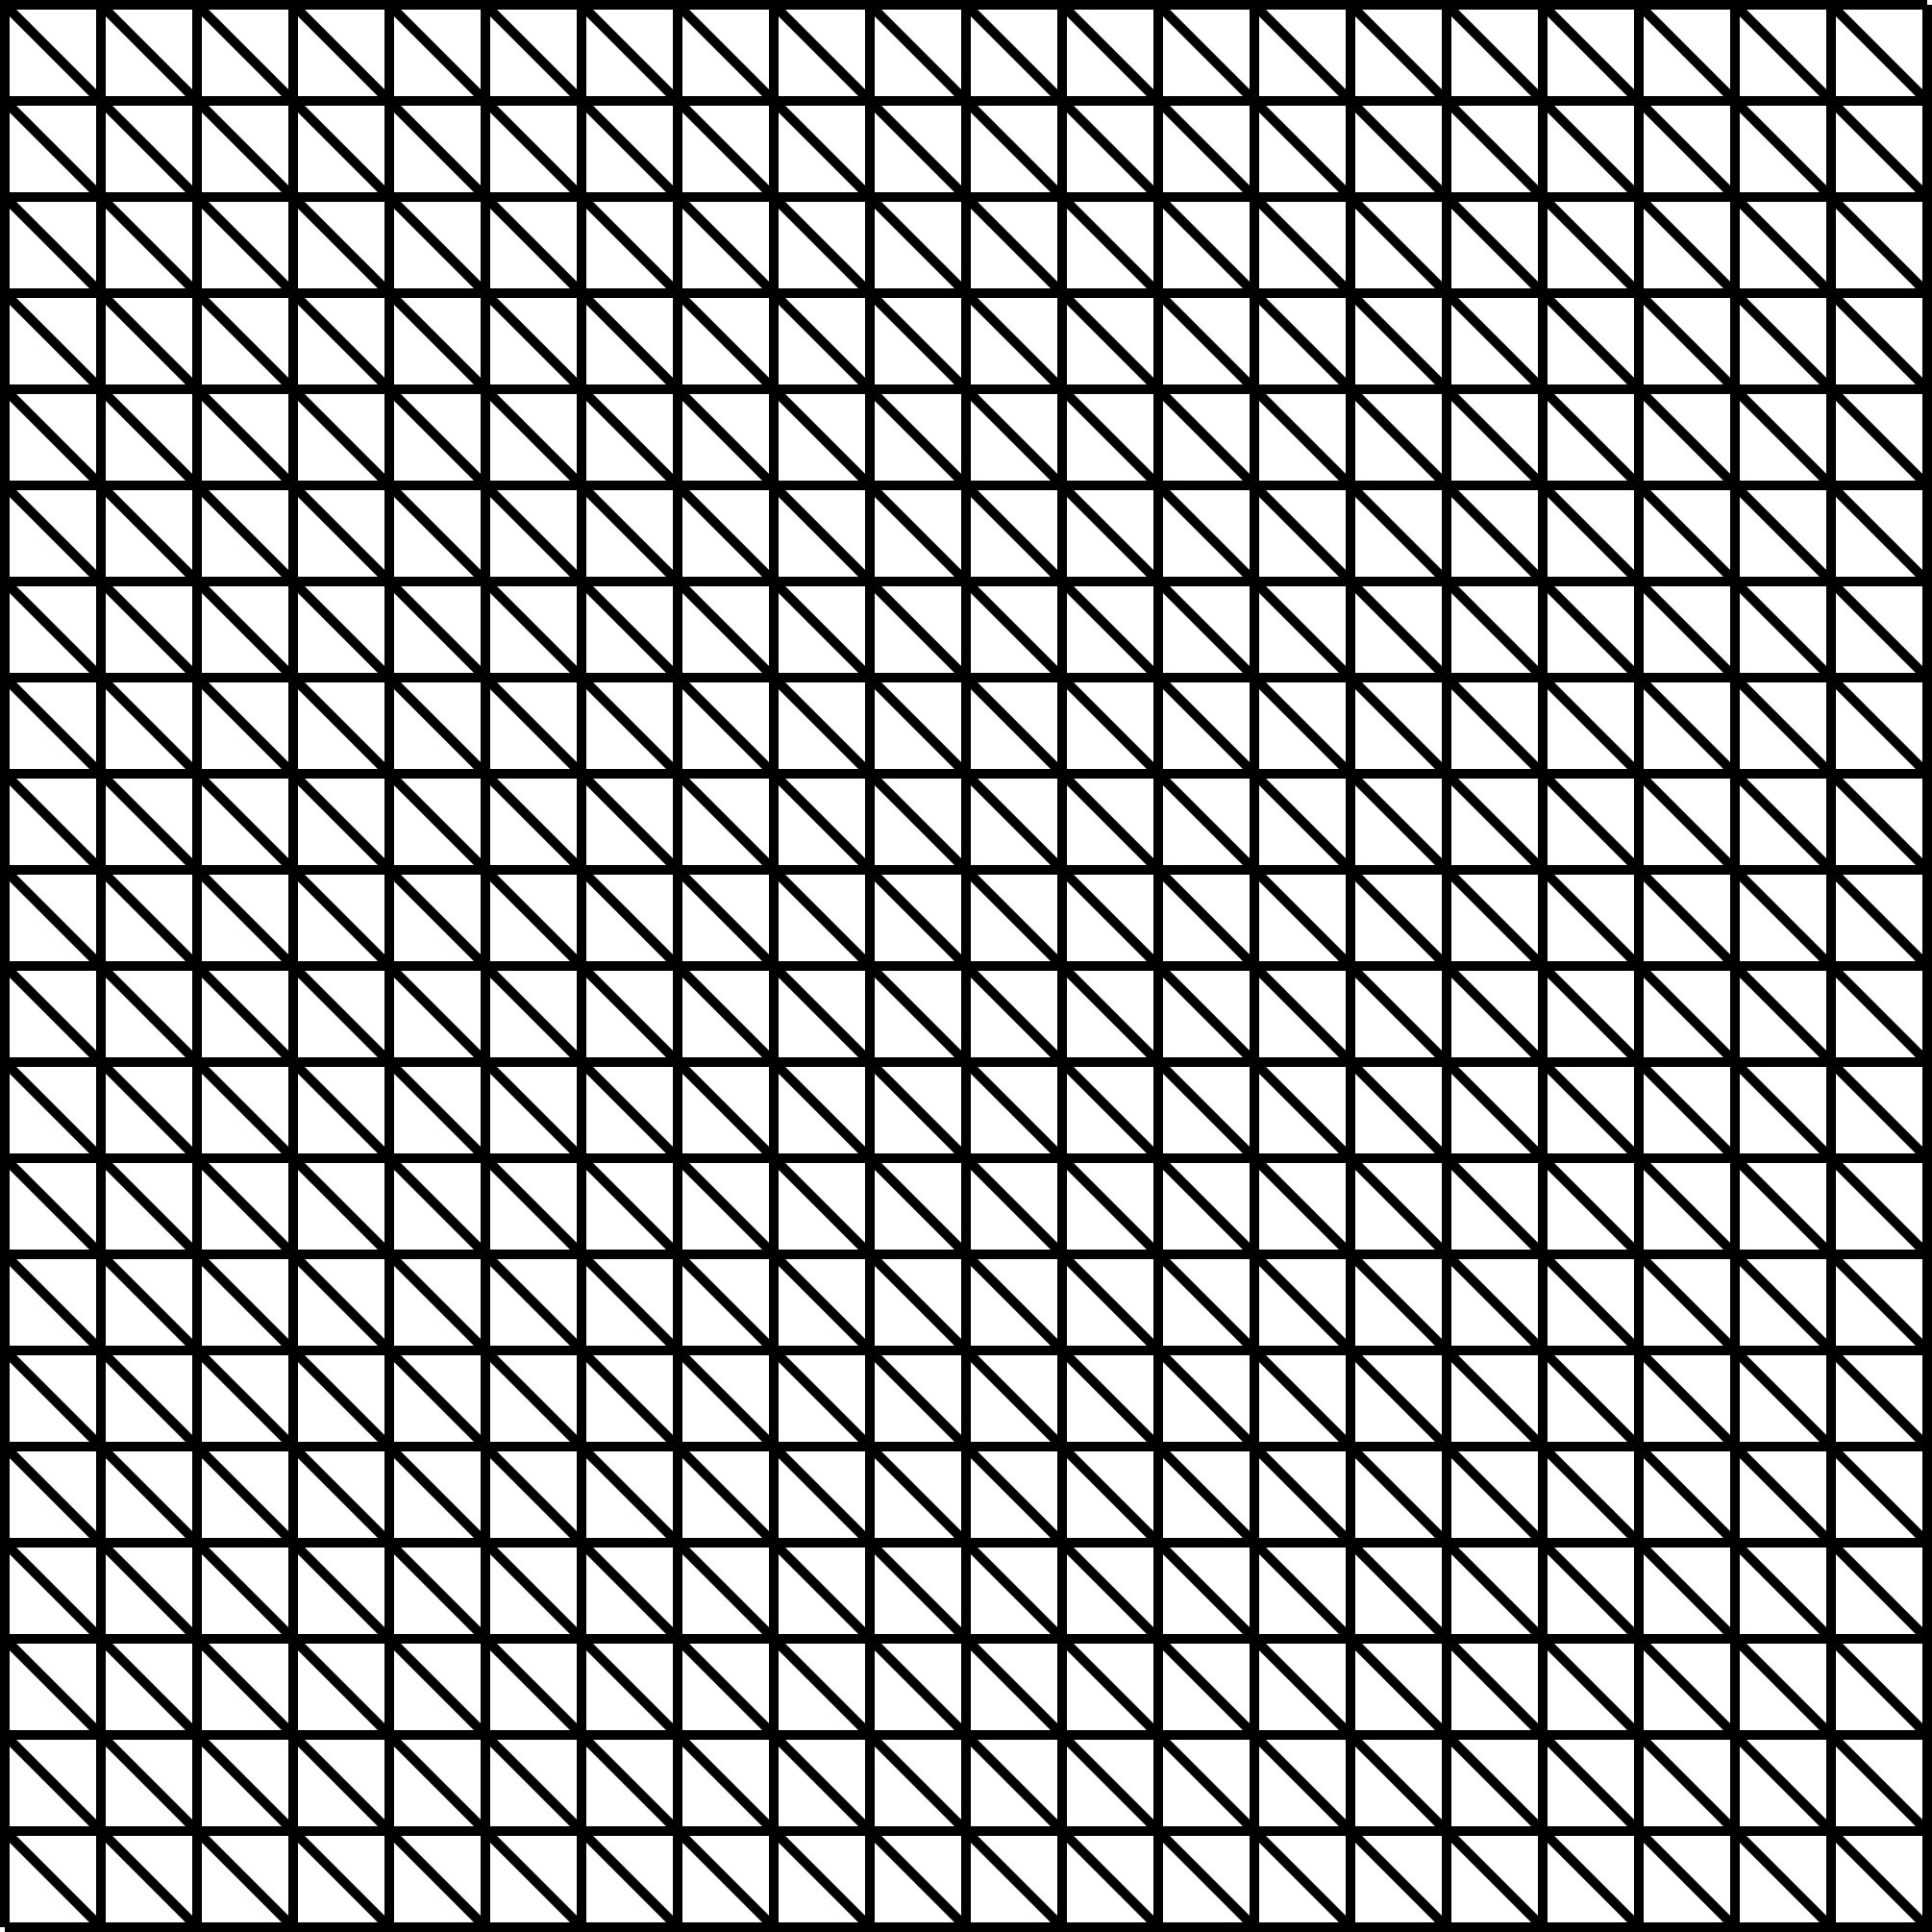
\includegraphics[width=\linewidth]
		{data/synthetic_meshes/square_tesselation_2tri_Dirac_delta_10_v441_f800_wireframe.png}
		\caption{$r=10$, wireframe}\label{fig:sq2.d}
	\end{subfigure}
	\begin{subfigure}[b]{0.32\linewidth}
		\includegraphics[width=\linewidth]
		{data/synthetic_meshes/square_tesselation_2tri_Dirac_delta_10_v441_f800_funcvals_0iter.png}
		\caption{$r=10$, $c=0$}\label{fig:sq2.e}
	\end{subfigure}
	\begin{subfigure}[b]{0.32\linewidth}
		\includegraphics[width=\linewidth]
		{data/synthetic_meshes/square_tesselation_2tri_Dirac_delta_10_v441_f800_funcvals_100iter.png}
		\caption{$r=10$, $c=100$}\label{fig:sq2.f}
	\end{subfigure}
\end{figure}
